\section{Sistemi retroazionati: criterio di Nyquist e margini di stabilità}

\subsection{Buona connessione}

\begin{definition}
  Il sistema retroazionato è detto ben connesso se:
  \begin{equation}
    \lim_{s\to\infty} 1 + L(s) \neq 0
  \end{equation}
\end{definition}


\subsection{Criterio di Nyquist}

\begin{figure}[h!]
  \centering
  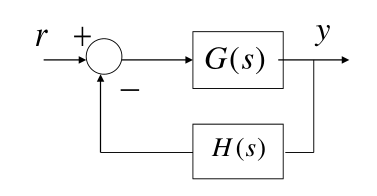
\includegraphics[width=0.5\textwidth]{./images/retroazione.png}
  \caption{Schema di retroazione}
  \label{fig:retroazione2}
\end{figure}

Come da esempio la funzione di trasferimento di un sistema retroazionato è:
\begin{equation}
  T(s) = \frac{G(s)}{1 + G(s)H(s)}
\end{equation}


Il sistema retrazionato è stabile se e solo se:
\begin{equation}
  1 + G(s)H(s) = 0
\end{equation}
Ha \textbf{tutte radici a parte reale negativa}.




\subsection{Teorema dell'indice logaritmico}
Sia \( \Gamma \) una curva chiusa semplice del piano complesso e \( D \) la
regione ad essa interna ( \( \Gamma = \partial D \) ). Sia \( F(s) \) una
funzione analitica su \( \Gamma \) e su \( D \) ad eccezione di un numero
finito di poli appartenenti a \( D \). Inoltre, \( F(s) \) non abbia zeri su \(
\Gamma \). Vale quindi la relazione: \begin{equation} \frac{1}{2\pi} \Delta
\arg F(s) = n_z - n_p \end{equation} dove \( \Delta \arg F(s) \) denota la
variazione dell'argomento di \( F(s) \) al variare di \( s \) lungo \( \Gamma
\) per un giro completo in senso antiorario, ed \( n_z \) e \( n_p \) sono
rispettivamente il numero degli zeri e dei poli di \( F(s) \) su \( D \),
computati con le loro molteplicità.





Assumendo la percorrenza di $\Gamma$ \textbf{in senso antiorario}:
\begin{theorem}
  Numero di giri \textbf{in senso antiorario} della curva immagine
  intorno all'origine:
  \begin{equation}
    n_{z} - n_{p}
  \end{equation}
\end{theorem}



Assumendo la percorrenza di $\Gamma$ \textbf{in senso orario}:
\begin{theorem}
  Numero di giri \textbf{in senso orario} della curva immagine
  intorno all'origine:
  \begin{equation}
    n_{z} - n_{p}
  \end{equation}
\end{theorem}



\textbf{Il diagramma polare di $G(s)H(s)$ non deve attraversare il punto
$-1+j0$}.

Ecco alcune definizioni:
\begin{itemize}
  \item $n_z :=$ numero di zeri di $1 + G(s)H(s)$ in $\mathbb{C}_{+}$
  \item $n_p :=$ numero di poli di $1 + G(s)H(s)$ in $\mathbb{C}_{+}$
  \item $\Psi := $ numero di giri in senso orario della curva immagine
    intorno all'origine
\end{itemize}

Assunto che il diagramma polare non attraversi il punto $-1+j0$, vale:
\begin{equation}
  \Psi = n_z - n_p
\end{equation}


\begin{definition}[Criterio di Nyquist]
  Condizione necessaria e sufficiente affinché il sistema in retroazione sia
  asintoticamente stabile è che il diagramma polare completo non tocchi il
  punto critico $-1$ ma lo circondi tante volte in senso antiorario quanti sono
  i poli del guadagno di anello con parte reale positiva. 
\end{definition}


\begin{definition}[Caso particolare] Nell’ipotesi che il guadagno di anello
  non abbia poli a parte reale positiva, condizione necessaria e sufficiente
  affinché il sistema in retroazione sia asintoticamente stabile è che il
  diagramma polare completo non tocchi né circondi il punto critico $-1$.
\end{definition}


\subsection{Margine di stabilità}

\begin{equation}
  M_A := \frac{1}{|G(j\omega_p)H(j\omega_p)|}
  \label{eq:margine_stabilita}
\end{equation}

Dove $\omega_p$ è la pulsazione di attraversamento del diagramma polare del
punto critico $-1$.

\begin{equation}
  \omega_p \implies \arg G(j\omega_p)H(j\omega_p) = - \pi
\end{equation}

Mentre il margine di fase è:
\begin{equation}
  M_F := \pi - |\varphi_c|
  \label{eq:margine_fase}
\end{equation}

Dove $\varphi_c$ è:
\begin{equation}
\varphi_c = \arg G(j\omega_c)H(j\omega_c)
\end{equation}

$\omega_c$ è:
\begin{equation}
  |G(j\omega_c)H(j\omega_c)| = 1
\end{equation}



